% 2006 年全国卷Ⅱ文科第 22 题：抛物线与两条切线
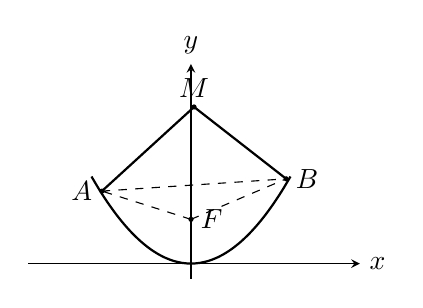
\begin{tikzpicture}[>=stealth,scale=0.78]
  \draw[->] (-2.65,0)--(2.75,0) node[right] {$x$};
  \draw[->] (0,-0.25)--(0,3.25) node[above] {$y$};
  \draw[thick] plot[smooth,domain=-2.25:2.25] ({0.72*\x},{0.28*\x*\x});
  \coordinate (F) at (0,0.72);
  \coordinate (A) at (-1.45,1.18);
  \coordinate (B) at (1.55,1.38);
  \coordinate (M) at (0.05,2.55);
  \draw[dashed] (A)--(B) (F)--(A) (F)--(B);
  \draw[thick] (A)--(M) (B)--(M);
  \fill (F) circle (1.2pt) node[right] {$F$};
  \fill (A) circle (1.2pt) node[left] {$A$};
  \fill (B) circle (1.2pt) node[right] {$B$};
  \fill (M) circle (1.2pt) node[above] {$M$};
\end{tikzpicture}
